\documentclass[tikz,border=5pt]{standalone}
\usepackage{tikz}
\usepackage{lmodern}
\usetikzlibrary{shapes,arrows,positioning,calc,fit}

\begin{document}
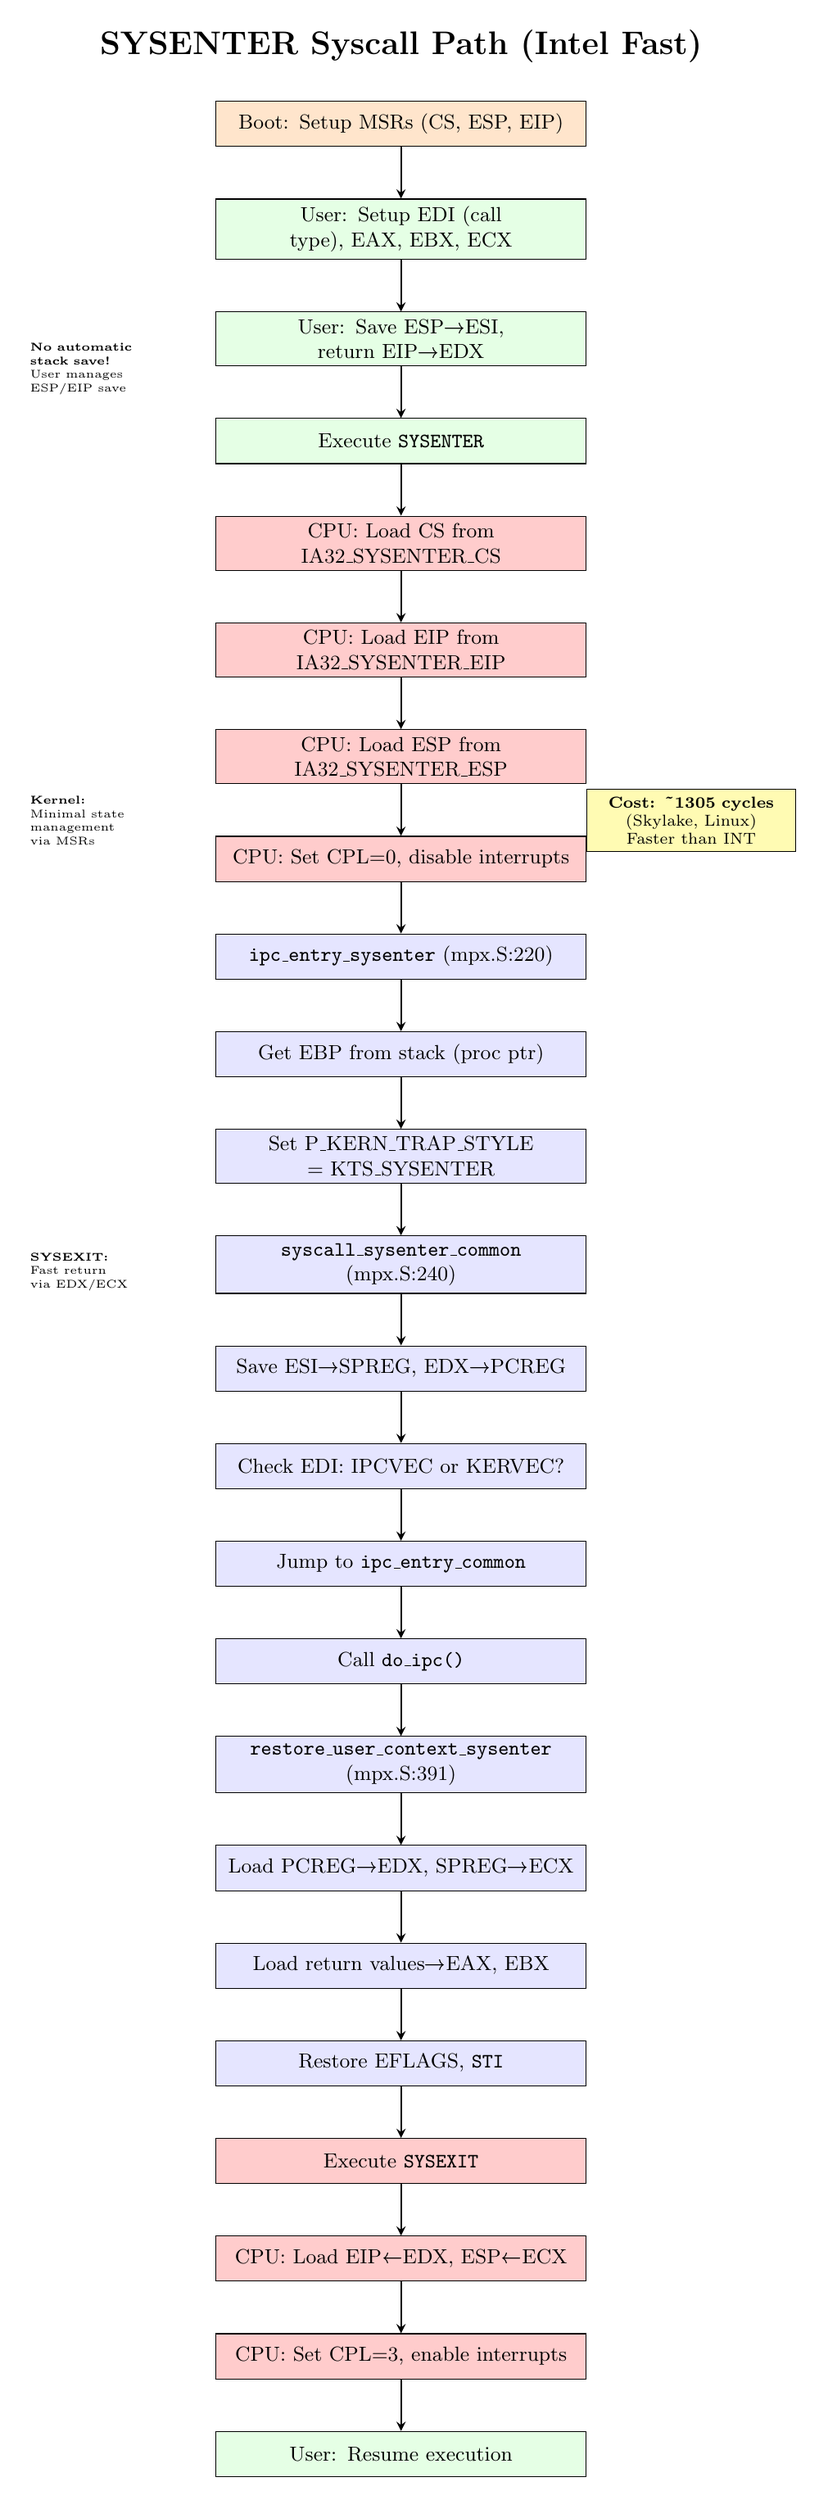
\begin{tikzpicture}[
    node distance=0.8cm,
    box/.style={rectangle, draw, fill=blue!10, text width=5.5cm, align=center, minimum height=0.7cm, font=\small},
    hw/.style={rectangle, draw, fill=red!20, text width=5.5cm, align=center, minimum height=0.7cm, font=\small},
    user/.style={rectangle, draw, fill=green!10, text width=5.5cm, align=center, minimum height=0.7cm, font=\small},
    arrow/.style={->,>=stealth,thick}
]

% Title
\node[font=\Large\bfseries] at (0,0) {SYSENTER Syscall Path (Intel Fast)};

% MSR Setup (boot time)
\node[box, fill=orange!20] (msr) at (0,-1.2) {Boot: Setup MSRs (CS, ESP, EIP)};

% User space prep
\node[user] (user1) [below=of msr] {User: Setup EDI (call type), EAX, EBX, ECX};
\node[user] (user2) [below=of user1] {User: Save ESP→ESI, return EIP→EDX};
\node[user] (user3) [below=of user2] {Execute \texttt{SYSENTER}};

% Hardware actions
\node[hw] (hw1) [below=of user3] {CPU: Load CS from IA32\_SYSENTER\_CS};
\node[hw] (hw2) [below=of hw1] {CPU: Load EIP from IA32\_SYSENTER\_EIP};
\node[hw] (hw3) [below=of hw2] {CPU: Load ESP from IA32\_SYSENTER\_ESP};
\node[hw] (hw4) [below=of hw3] {CPU: Set CPL=0, disable interrupts};

% Kernel entry
\node[box] (kern1) [below=of hw4] {\texttt{ipc\_entry\_sysenter} (mpx.S:220)};
\node[box] (kern2) [below=of kern1] {Get EBP from stack (proc ptr)};
\node[box] (kern3) [below=of kern2] {Set P\_KERN\_TRAP\_STYLE = KTS\_SYSENTER};
\node[box] (kern4) [below=of kern3] {\texttt{syscall\_sysenter\_common} (mpx.S:240)};
\node[box] (kern5) [below=of kern4] {Save ESI→SPREG, EDX→PCREG};
\node[box] (kern6) [below=of kern5] {Check EDI: IPCVEC or KERVEC?};
\node[box] (kern7) [below=of kern6] {Jump to \texttt{ipc\_entry\_common}};
\node[box] (kern8) [below=of kern7] {Call \texttt{do\_ipc()}};

% Return path
\node[box] (ret1) [below=of kern8] {\texttt{restore\_user\_context\_sysenter} (mpx.S:391)};
\node[box] (ret2) [below=of ret1] {Load PCREG→EDX, SPREG→ECX};
\node[box] (ret3) [below=of ret2] {Load return values→EAX, EBX};
\node[box] (ret4) [below=of ret3] {Restore EFLAGS, \texttt{STI}};
\node[hw] (hw5) [below=of ret4] {Execute \texttt{SYSEXIT}};
\node[hw] (hw6) [below=of hw5] {CPU: Load EIP←EDX, ESP←ECX};
\node[hw] (hw7) [below=of hw6] {CPU: Set CPL=3, enable interrupts};
\node[user] (user4) [below=of hw7] {User: Resume execution};

% Arrows
\foreach \i/\j in {msr/user1, user1/user2, user2/user3, user3/hw1, hw1/hw2, hw2/hw3, hw3/hw4, hw4/kern1, kern1/kern2, kern2/kern3, kern3/kern4, kern4/kern5, kern5/kern6, kern6/kern7, kern7/kern8, kern8/ret1, ret1/ret2, ret2/ret3, ret3/ret4, ret4/hw5, hw5/hw6, hw6/hw7, hw7/user4} {
    \draw[arrow] (\i) -- (\j);
}

% Side annotations
\node[font=\tiny, text width=2.5cm, align=left] at (-4.5,-5) {
    \textbf{No automatic}\\
    \textbf{stack save!}\\
    User manages\\
    ESP/EIP save
};

\node[font=\tiny, text width=2.5cm, align=left] at (-4.5,-12) {
    \textbf{Kernel:}\\
    Minimal state\\
    management\\
    via MSRs
};

\node[font=\tiny, text width=2.5cm, align=left] at (-4.5,-19) {
    \textbf{SYSEXIT:}\\
    Fast return\\
    via EDX/ECX
};

% Cycle cost annotation
\node[font=\scriptsize, fill=yellow!30, draw, text width=3cm, align=center] at (4.5,-12) {
    \textbf{Cost: \textasciitilde1305 cycles}\\
    (Skylake, Linux)\\
    Faster than INT
};

\end{tikzpicture}
\end{document}
